
%%%%%%%%%%%%%%%%%%%%%%%%%%%%%%%%%%%%%%%%%%%%%%%%%%%%%%%%
%
% Copyright (c) 2003-2009 by University of Queensland
% Earth Systems Science Computational Center (ESSCC)
% http://www.uq.edu.au/esscc
%
% Primary Business: Queensland, Australia
% Licensed under the Open Software License version 3.0
% http://www.opensource.org/licenses/osl-3.0.php
%
%%%%%%%%%%%%%%%%%%%%%%%%%%%%%%%%%%%%%%%%%%%%%%%%%%%%%%%%

\section{One Dimensional Heat Diffusion in an Iron Rod}
\sslist{onedheatdiff001.py and cblib.py}
%\label{Sec:1DHDv0}
We will start by examining a simple one dimensional heat diffusion example. This problem will provide a good launch pad to build our knowledge of \esc and how to solve simple partial differential equations (PDEs)\footnote{Wikipedia provides an excellent and comprehensive introduction to \textit{Partial Differential Equations} \url{http://en.wikipedia.org/wiki/Partial_differential_equation}, however their relevance to \esc and implementation should become a clearer as we develop our understanding further into the cookbook.}

\begin{figure}[h!]
\centerline{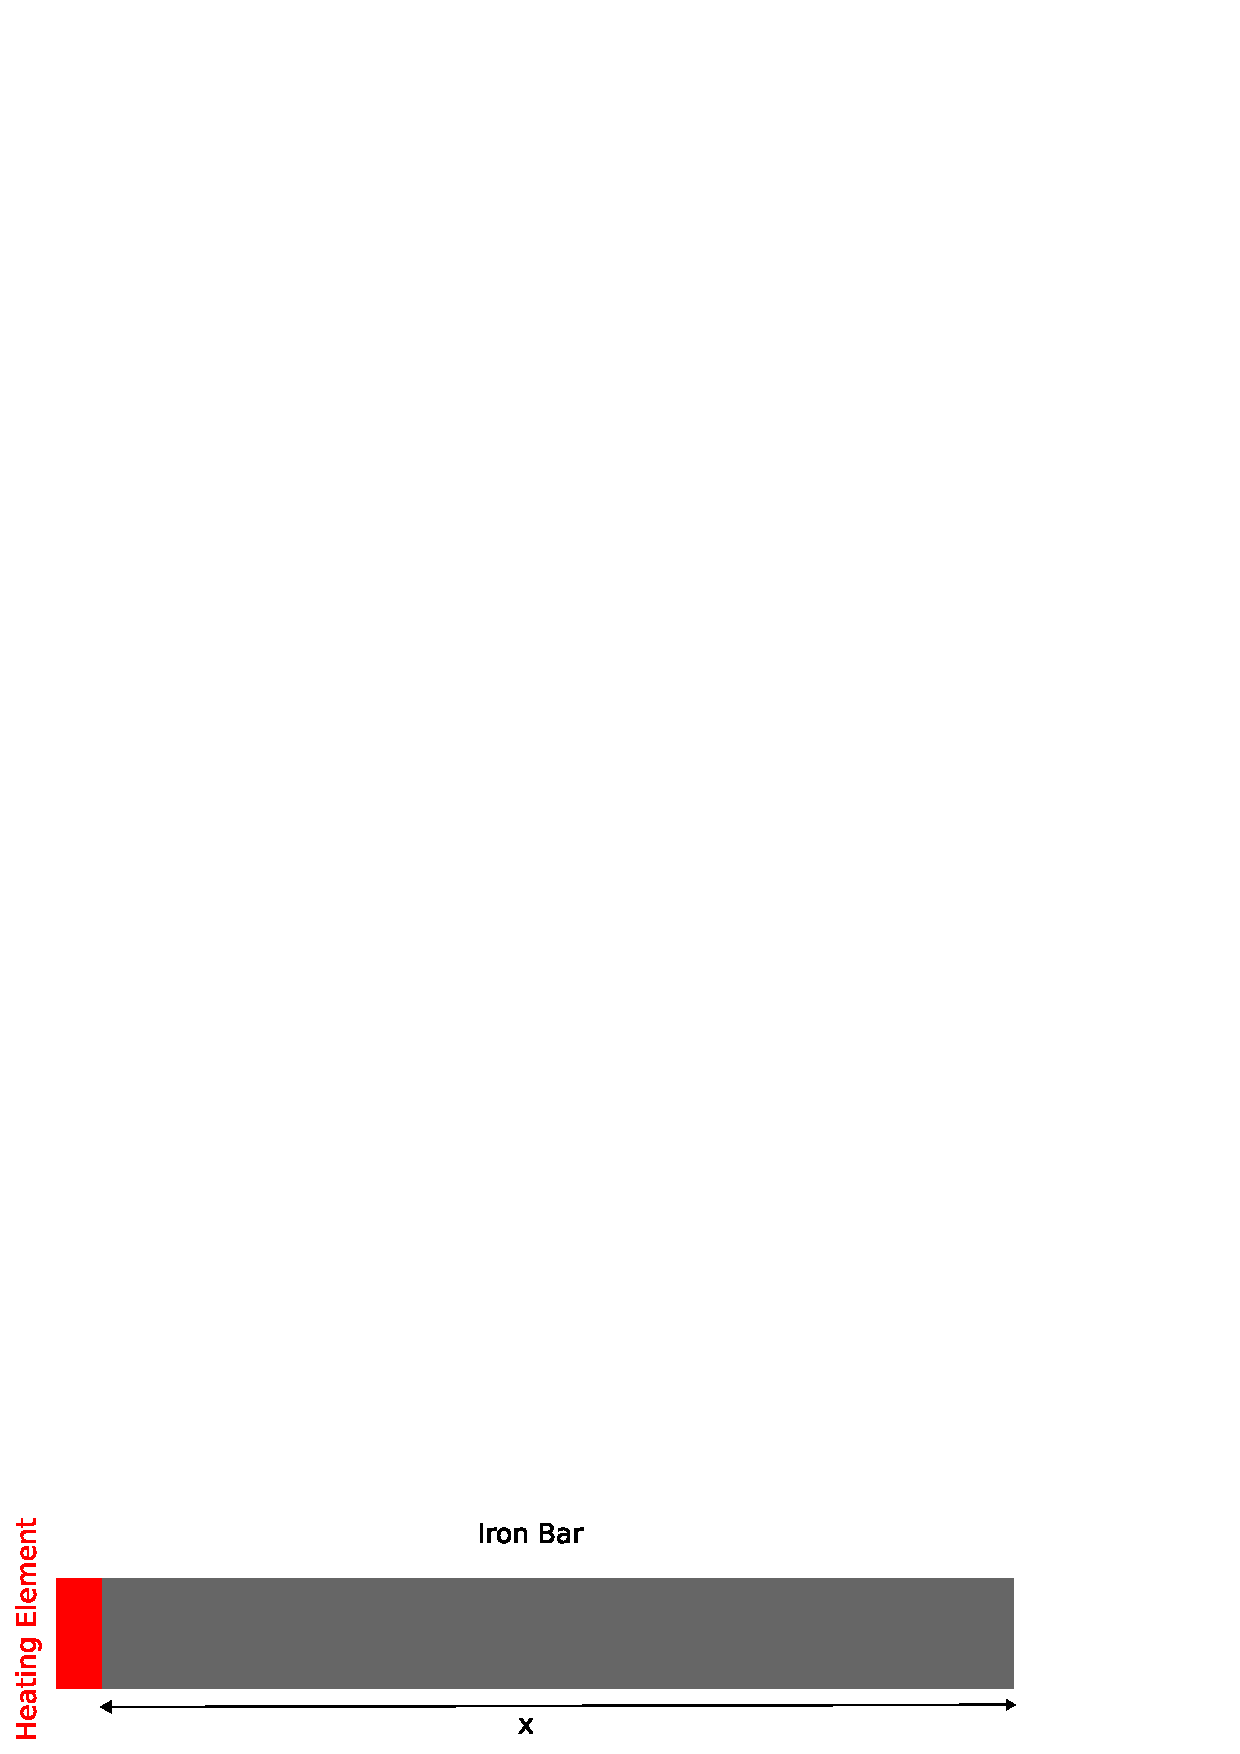
\includegraphics[width=4.in]{figures/onedheatdiff}}
\caption{One dimensional model of an Iron bar.}
\label{fig:onedhdmodel}
\end{figure}
The first model consists of a simple cold iron bar at a constant temperature of zero \reffig{fig:onedhdmodel}. The bar is perfectly insulated on all sides with a heating element at one end. Intuition tells us that as heat is applied; energy will disperse along the bar via conduction. With time the bar will reach a constant temperature equivalent to the heat source.

\subsection{1D Heat Diffusion Equation}
We can model the heat distribution of this problem over time using the one dimensional heat diffusion equation\footnote{A detailed discussion on how the heat diffusion equation is derived can be found at \url{http://online.redwoods.edu/instruct/darnold/DEProj/sp02/AbeRichards/paper.pdf}};
which is defined as:
\begin{equation}
\rho c\hackscore p \frac{\partial T}{\partial t} - \kappa \frac{\partial^{2} T}{\partial x^{2}} = q\hackscore H 
\label{eqn:hd}
\end{equation}
where $\rho$ is the material density, $c\hackscore p$ is the specific heat and $\kappa$ is the thermal conductivity constant for a given material\footnote{A list of some common thermal conductivities is available from Wikipedia \url{http://en.wikipedia.org/wiki/List_of_thermal_conductivities}}. 
The heat source is defined by the right hand side of \ref{eqn:hd} as $q\hackscore{H}$; this can take the form of a constant or a function of time and space. For example $q\hackscore{H} = Te^{-\gamma t}$ where we have the output of our heat source decaying with time. There are also two partial derivatives in \ref{eqn:hd}; $\frac{\partial T}{\partial t}$ describes the change in temperature with time while $\frac{\partial ^2 T}{\partial x^2}$ is the spatial change of temperature. As there is only a single spatial dimension to our problem, our temperature solution $T$ is only dependent on the time $t$ and our position along the iron bar $x$.

\subsection{Escript, PDEs and The General Form}
Potentially, it is now possible to solve \ref{eqn:hd} analytically and this would produce an exact solution to our problem. However, it is not always possible or practical to solve a problem this way. Alternatively, computers can be used to solve these kinds of problems when a large number of sums or a more complex visualisation is required. To do this, a numerical approach is required - \esc can help us here -  and it becomes necessary to discretize the equation so that we are left with a finite number of equations for a finite number of spatial and time steps in the model. While discretization introduces approximations and a degree of error, we find that a sufficiently sampled model is generally accurate enough for the requirements of the modeller.

\esc interfaces with any given PDE via a general form. In this example we will illustrate a simpler version of the full linear PDE general form which is available in the \esc user's guide. A simplified form that suits our heat diffusion problem\footnote{In the form of the \esc users guide which using the Einstein convention is written as 
$-(A\hackscore{jl} u\hackscore{,l})\hackscore{,j}+D u =Y$}
is described by;
\begin{equation}\label{eqn:commonform nabla}
-\nabla\cdot(A\cdot\nabla u) + Du = f
\end{equation}
where $A$, $D$ and $f$ are known values. The symbol $\nabla$ which is called the \textit{Nabla operator} or \textit{del operator} represents
the spatial derivative of its subject - in this case $u$. Lets assume for a moment that we deal with a one-dimensional problem then ;
\begin{equation}
\nabla = \frac{\partial}{\partial x}
\end{equation}
and we can write \ref{eqn:commonform nabla} as;
\begin{equation}\label{eqn:commonform}
-A\frac{\partial^{2}u}{\partial x^{2}} + Du = f
\end{equation}
if $A$ is constant then  \ref{eqn:commonform} is consistent with our heat diffusion problem in \ref{eqn:hd} with the exception of $u$. Thus when comparing equations \ref{eqn:hd} and \ref{eqn:commonform} we see that;
\begin{equation}
A = \kappa; D = \rho c \hackscore{p}; f = q \hackscore{H}
\end{equation}

We can write the partial $\frac{\partial T}{\partial t}$ in terms of $u$ by discretising the time of our solution. The method we will use is the Backwards Euler approximation, which states;
\begin{equation}
\frac{\partial f(x)}{\partial x} \approx \frac{f(x+h)-f(x)}{h}
\label{eqn:beuler}
\end{equation}
where h is the the discrete step size $\Delta x$.
Now if the temperature $T(t)$ is substituted in by letting $f(x) = T(t)$ then from \ref{eqn:beuler} we see that;
\begin{equation}
T'(t) \approx \frac{T(t+h) - T(t)}{h}
\end{equation}
which can also be written as;
\begin{equation}
\frac{\partial T^{(n)}}{\partial t} \approx \frac{T^{(n)} - T^{(n-1)}}{h}
\label{eqn:Tbeuler}
\end{equation}
where $n$ denotes the n\textsuperscript{th} time step. Substituting \ref{eqn:Tbeuler} into \ref{eqn:hd} we get;
\begin{equation}
\frac{\rho c\hackscore p}{h} (T^{(n)} - T^{(n-1)}) - \kappa \frac{\partial^{2} T}{\partial x^{2}} = q\hackscore H 
\label{eqn:hddisc}
\end{equation}
To fit our simplified general form we can rearrange \ref{eqn:hddisc};
\begin{equation}
\frac{\rho c\hackscore p}{h} T^{(n)} - \kappa \frac{\partial^2 T^{(n)}}{\partial x^2} = q\hackscore H +  \frac{\rho c\hackscore p}{h} T^{(n-1)}
\label{eqn:hdgenf}
\end{equation}
The PDE is now in a form that satisfies \refEq{eqn:commonform nabla} which is required for \esc to solve our PDE. This can be done by generating a solution for successive increments in the time nodes $t^{(n)}$ where 
$t^{(0)}=0$ and  $t^{(n)}=t^{(n-1)}+h$ where $h>0$ is the step size and assumed to be constant. 
In the following the upper index ${(n)}$ refers to a value at time $t^{(n)}$. Finally, by comparing \ref{eqn:hdgenf} with \ref{eqn:commonform} it can be seen that;
\begin{equation}
A = \kappa; D = \frac{\rho c \hackscore{p}}{h}; f = q \hackscore{H} + \frac{\rho c\hackscore p}{h} T^{(n-1)}
\end{equation}

Now that the general form has been established, it can be submitted to \esc. Note that it is necessary to establish the state of our system at time zero or $T^{(n=0)}$. This is due to the time derivative approximation we have used from \ref{eqn:Tbeuler}. Our model stipulates a starting temperature in the iron bar of 0\textcelsius. Thus the temperature distribution is simply;
\begin{equation}
T(x,0) = T\hackscore{ref} = 0
\end{equation}
for all $x$ in the domain. 

\subsection{Boundary Conditions}
With the PDE sufficiently modified, consideration must now be given to the boundary conditions of our model. Typically there are two main types of boundary conditions known as Neumann and Dirichlet\footnote{More information on Boundary Conditions is available at Wikipedia \url{http://en.wikipedia.org/wiki/Boundary_conditions}}. In this example, we have utilised both conditions. Dirichlet is conceptually simpler and is used to prescribe a known value to the model on its boundary. This is like holding a snake by the tail; we know where the tail will be as we hold it however, we have no control over the rest of the snake. Dirichlet boundary conditions exist where we have applied our heat source. As the heat source is a constant, we can simulate its presence on that boundary. This is done by continuously resetting the temperature of the boundary, so that is is the same as the heat source.  

Neumann boundary conditions describe the radiation or flux normal to the boundary surface. This aptly describes our insulation conditions as we do not want to exert a constant temperature as with the heat source. However, we do want to prevent any loss of energy from the system. These natural boundary conditions can be described by specifying a radiation condition which prescribes the normal component of the flux $\kappa T\hackscore{,i}$ to be proportional
to the difference of the current temperature to the surrounding temperature $T\hackscore{ref}$; in general terms this is;
\begin{equation}
 \kappa T\hackscore{,i} \hat{n}\hackscore i = \eta (T\hackscore{ref}-T) 
\label{eqn:hdbc}
\end{equation}
and simplified to our one dimensional model we have;
\begin{equation}
\kappa \frac{\partial T}{\partial dx} \hat{n}\hackscore x = \eta (T\hackscore{ref}-T) 
\end{equation}
where $\eta$ is a given material coefficient depending on the material of the block and the surrounding medium and $\hat{n}\hackscore i$ is the $i$-th component of the outer normal field \index{outer normal field} at the surface of the domain. These two conditions form a boundary value problem that has to be solved for each time step. Due to the perfect insulation in our model we can set $\eta = 0$ which results in zero flux - no energy in or out - we do not need to worry about the Neumann terms of the general form for this example.

\subsection{A \textit{1D} Clarification}
It is necessary for clarification that we revisit the general PDE from \refeq{eqn:commonform nabla} under the light of a two dimensional domain. \esc is inherently designed to solve problems that are greater than one dimension and so \ref{eqn:commonform nabla} needs to be read as a higher dimensional problem. In the case of two spatial dimensions the \textit{Nabla operator} has in fact two components $\nabla = (\frac{\partial}{\partial x}, \frac{\partial}{\partial y})$. In full, \ref{eqn:commonform nabla} assuming a constant coefficient $A$, takes the form;
\begin{equation}\label{eqn:commonform2D}
-A\hackscore{00}\frac{\partial^{2}u}{\partial x^{2}} 
-A\hackscore{01}\frac{\partial^{2}u}{\partial x\partial y} 
-A\hackscore{10}\frac{\partial^{2}u}{\partial y\partial x} 
-A\hackscore{11}\frac{\partial^{2}u}{\partial y^{2}} 
+ Du = f
\end{equation}
Notice that for the higher dimensional case $A$ becomes a matrix. It is also
important to notice that the usage of the Nabla operator creates
a compact formulation which is also independent from the spatial dimension. 
So to make the general PDE~\ref{eqn:commonform2D} one dimensional as
shown in~\ref{eqn:commonform} we need to set
\begin{equation}
A\hackscore{00}=A; A\hackscore{01}=A\hackscore{10}=A\hackscore{11}=0
\end{equation}

\subsection{Developing a PDE Solution Script}
To solve \ref{eqn:hd} we will write a simple python script which uses the \modescript, \modfinley and \modmpl modules. At this point we assume that you have some basic understanding of the python programming language. If not there are some pointers and links available in Section \ref{sec:escpybas} .

Our goal here is to develop a script for \esc that will solve the heat equation at successive time steps for a predefined period using our general form \ref{eqn:hdgenf}. Firstly it is necessary to import all the libraries\footnote{The libraries contain predefined scripts that are required to solve certain problems, these can be simple like sin and cos functions or more complicated like those from our \esc library.} 
that we will require.
\begin{python}
from esys.escript import *
# This defines the LinearPDE module as LinearPDE
from esys.escript.linearPDEs import LinearPDE 
# This imports the rectangle domain function from finley.
from esys.finley import Rectangle 
# A useful unit handling package which will make sure all our units
# match up in the equations under SI.
from esys.escript.unitsSI import * 
import pylab as pl #Plotting package.
import numpy as np #Array package.
import os #This package is necessary to handle saving our data.
\end{python}
It is generally a good idea to import all of the \modescript library, although if you know the packages you need you can specify them individually. The function \verb|LinearPDE| has been imported for ease of use later in the script. \verb|Rectangle| is going to be our type of domain. The package \verb unitsSI  is a module of \esc that provides support for units definitions with our variables; and the \verb|os| package is needed to handle file outputs once our PDE has been solved. \verb pylab  and \verb numpy  are modules developed independently of \esc. They are used because they have efficient plotting and array handling capabilities.

Once our library dependencies have been established, defining the problem specific variables is the next step. In general the number of variables needed will vary between problems. These variables belong to two categories. They are either directly related to the PDE and can be used as inputs into the \esc solver, or they are script variables used to control internal functions and iterations in our problem. For this PDE there are a number of constants which will need values. Firstly, the domain upon which we wish to solve our problem needs to be defined. There are many different types of domains in \modescript which we will demonstrate in later tutorials but for our iron rod, we will simply use a rectangular domain. 

Using a rectangular domain simplifies our rod which would be a \textit{3D} object, into a single dimension. The iron rod will have a lengthways cross section that looks like a rectangle.  As a result we do not need to model the volume of the rod because a cylinder is symmetrical about its centre. There are four arguments we must consider when we decide to create a rectangular domain, the model \textit{length}, \textit{width} and \textit{step size} in each direction. When defining the size of our problem it will help us determine appropriate values for our domain arguments. If we make our dimensions large but our step sizes very small we will to a point, increase the accuracy of our solution. Unfortunately we also increase the number of calculations that must be solved per time step. This means more computational time is required to produce a solution. In our \textit{1D} problem we will define our bar as being 1 metre long. An appropriate \verb|ndx| would be 1 to 10\% of the length. Our \verb|ndy| need only be 1, This is because our problem stipulates no partial derivatives in the $y$ direction so the temperature does not vary with $y$. Thus the domain parameters can be defined as follows; note we have used the \verb unitsSI  convention to make sure all our input units are converted to SI.
\begin{python}
#Domain related.
mx = 1*m #meters - model length
my = .1*m #meters - model width
ndx = 100 # mesh steps in x direction 
ndy = 1 # mesh steps in y direction - one dimension means one element
\end{python}
The material constants and the temperature variables must also be defined. For the iron rod in the model they are defined as:
\begin{python}
#PDE related
q=200. * Celsius #Kelvin - our heat source temperature
Tref = 0. * Celsius #Kelvin - starting temp of iron bar
rho = 7874. *kg/m**3 #kg/m^{3} density of iron
cp = 449.*J/(kg*K) #j/Kg.K thermal capacity
rhocp = rho*cp
kappa = 80.*W/m/K #watts/m.Kthermal conductivity
\end{python}
Finally, to control our script we will have to specify our timing controls and where we would like to save the output from the solver. This is simple enough:
\begin{python}
t=0 #our start time, usually zero
tend=5.*minute #seconds - time to end simulation
outputs = 200 # number of time steps required.
h=(tend-t)/outputs #size of time step
#user warning statement
print "Expected Number of time outputs is: ", (tend-t)/h
i=0 #loop counter
#the folder to put our outputs in, leave blank "" for script path 
save_path="data/onedheatdiff001"
\end{python}
Now that we know our inputs we will build a domain using the \verb Rectangle() function from \verb finley . The four arguments allow us to define our domain \verb rod  as:
\begin{python}
#generate domain using rectangle
rod = Rectangle(l0=mx,l1=my,n0=ndx, n1=ndy)
\end{python}
\verb rod  now describes a domain in the manner of Section \ref{ss:domcon}. As we define our variables, various function spaces will be created to accomodate them. There is an easy way to extract finite points from the domain \verb|rod| using the domain property function \verb|getX()| . This function sets the vertices of each cell as finite points to solve in the solution. If we let \verb|x| be these finite points, then;
\begin{python}
#extract finite points - the solution points
x=rod.getX()
\end{python}
The data locations of specific function spaces can be returned in a similar manner by extracting the relevent function space from the domain followed by the \verb .getX()  operator.

With a domain and all our required variables established, it is now possible to set up our PDE so that it can be solved by \esc. The first step is to define the type of PDE that we are trying to solve in each time step. In this example it is a single linear PDE\footnote{in comparison to a system of PDEs which will be discussed later.}. We also need to state the values of our general form variables.
\begin{python}
mypde=LinearSinglePDE(rod)
mypde.setValue(A=kappa*kronecker(rod),D=rhocp/h)
\end{python}

In a few special cases it may be possible to decrease the computational time of the solver if our PDE is symmetric. Symmetry of a PDE is defined by;
\begin{equation}\label{eqn:symm}
A\hackscore{jl}=A\hackscore{lj}
\end{equation}
Symmetry is only dependent on the $A$ coefficient in the general form and the others $D$ and $d$ as well as the RHS coefficients $Y$ and $y$ may take any value. From the above definition we can see that our PDE is symmetric. The \verb LinearPDE  class provides the method \method{checkSymmetry} to check if the given PDE is symmetric. As our PDE is symmetrical we will enable symmetry via;
\begin{python}
 myPDE.setSymmetryOn()
\end{python}

We now need to specify our boundary conditions and initial values. The initial values required to solve this PDE are temperatures for each discrete point in our domain. We will set our bar to:
\begin{python}
 T = Tref
\end{python}
Boundary conditions are a little more difficult. Fortunately the escript solver will handle our insulated boundary conditions by default with a zero flux operator. However, we will need to apply our heat source $q_{H}$ to the end of the bar at $x=0$ . \esc makes this easy by letting us define areas in our domain. The finite points in the domain were previously defined as \verb x  and it is possible to set all of points that satisfy $x=0$ to \verb q  via the \verb whereZero()  function. There are a few \verb where  functions available in \esc. They will return a value \verb 1  where they are satisfied and \verb 0  where they are not. In this case our \verb qH  is only applied to the far LHS of our model as required.
\begin{python}
# ... set heat source: ....
qH=q*whereZero(x[0])
\end{python}

Finally we will initialise an iteration loop to solve our PDE for all the time steps we specified in the variable section. As the RHS of the general form is dependent on the previous values for temperature \verb T  across the bar this must be updated in the loop. Our output at each timestep is \verb T  the heat distribution and \verb totT  the total heat in the system.
\begin{python}
while t<=tend:
	i+=1 #increment the counter
	t+=h #increment the current time
	mypde.setValue(Y=qH+rhocp/h*T) #set variable PDE coefficients
	T=mypde.getSolution() #get the PDE solution
	totT = rhocp*T #get the total heat solution in the system
\end{python}

\subsection{Plotting the heat solutions} 
Visualisation of the solution can be achieved using \mpl a module contained with \pylab. We start by modifying our solution script from before. Prior to the \verb while  loop we will need to extract our finite solution points to a data object that is compatible with \mpl. First it is necessary to convert \verb x  to a list of tuples. These are then converted to a \numpy array and the $x$ locations extracted via an array slice to the variable \verb plx  .
\begin{python}
#convert solution points for plotting
plx = x.toListOfTuples() 
plx = np.array(plx) #convert to tuple to numpy array
plx = plx[:,0] #extract x locations
\end{python}
As there are two solution outputs, we will generate two plots and save each to a file for every time step in the solution. The following is appended to the end of the \verb while  loop and creates two figures. The first figure is for the temperature distribution, and the second the total temperature in the bar. Both cases are similar with a few minor changes for scale and labelling. We start by converting the solution to a tuple and then plotting this against our \textit{x coordinates} \verb plx  from before. The axis is then standardised and a title applied. The figure is then saved to a *.png file and cleared for the following iteration.
\begin{python}
	#establish figure 1 for temperature vs x plots
	tempT = T.toListOfTuples(scalarastuple=False)
	pl.figure(1) #current figure
	pl.plot(plx,tempT) #plot solution
		#define axis extents and title
	pl.axis([0,1.0,273.14990+0.00008,0.004+273.1499])
	pl.title("Temperature accross Rod")
		#save figure to file
	pl.savefig(os.path.join(save_path+"/tempT","rodpyplot%03d.png") %i)
	pl.clf() #clear figure
	
	#establish figure 2 for total temperature vs x plots and repeat
	tottempT = totT.toListOfTuples(scalarastuple=False)
	pl.figure(2)
	pl.plot(plx,tottempT)
	pl.axis([0,1.0,9.657E08,12000+9.657E08])
	pl.title("Total temperature accross Rod")
	pl.savefig(os.path.join(save_path+"/totT","ttrodpyplot%03d.png")%i)
	pl.clf()
\end{python}
\begin{figure}
\begin{center}
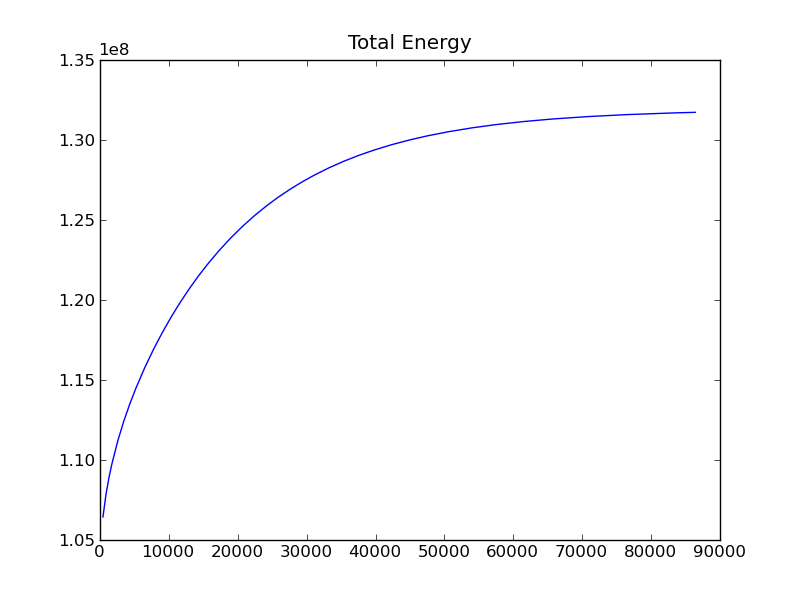
\includegraphics[width=4in]{figures/ttrodpyplot150}
\caption{Total temperature ($T$) distribution in rod at $t=150$}
\label{fig:onedheatout} 
\end{center}
\end{figure}

\subsubsection{Parallel scripts (MPI)}
In some of the example files for this cookbook the plot part of the script looks a little different.
For example,
\begin{python}
	pl.title("Total temperature accross Rod")
	if getMPIRankWorld() == 0:
	    pl.savefig(os.path.join(save_path+"/totT","ttrodpyplot%03d.png")%i)
	pl.clf()	
\end{python}

The additional \verb if  statement is not necessary for normal desktop use.
It becomes important for scripts run on parallel computers.
Its purpose is to ensure that only one copy of the file is written.
For more details on writing scripts for parallel computers please consult the \emph{user's guide}.

\subsection{Make a video} 
Our saved plots from the previous section can be cast into a video using the following command appended to the end of the script. \verb mencoder  is linux only however, and other platform users will need to use an alternative video encoder.
\begin{python}
# compile the *.png files to create two *.avi videos that show T change
# with time. This operation uses linux mencoder. For other operating 
# systems it is possible to use your favourite video compiler to
# convert image files to videos.

os.system("mencoder mf://"+save_path+"/tempT"+"/*.png -mf type=png:\
w=800:h=600:fps=25 -ovc lavc -lavcopts vcodec=mpeg4 -oac copy -o \
onedheatdiff001tempT.avi")

os.system("mencoder mf://"+save_path+"/totT"+"/*.png -mf type=png:\
w=800:h=600:fps=25 -ovc lavc -lavcopts vcodec=mpeg4 -oac copy -o \
onedheatdiff001totT.avi")
\end{python}
 
